% !TEX encoding = UTF-8 Unicode

\documentclass[aspectratio=169]{beamer}
\usepackage[utf8]{inputenc}

\usepackage{graphicx}
\graphicspath{{images/}}
\usepackage{tikz}

%% COLORS
\definecolor{UWRed}{HTML}{C5050C}
\setbeamercolor{structure}{fg=UWRed}
\setbeamercolor{title page}{fg=white}
\setbeamercolor{title}{fg=white}

%% LOGO on slides
\logo{
\includegraphics[height=10mm]{SMPH_color-flush.pdf}}

%% RM NAV SYMBOLS
\setbeamertemplate{navigation symbols}{}

%% FONTS
\setbeamerfont{title}{size=\Huge\bfseries}

\title{My title}
\subtitle{Subtitle}
\institute{University of Wisconsin--Madison}
\author{Myself \and Others}

\begin{document}

  {
    \usebackgroundtemplate{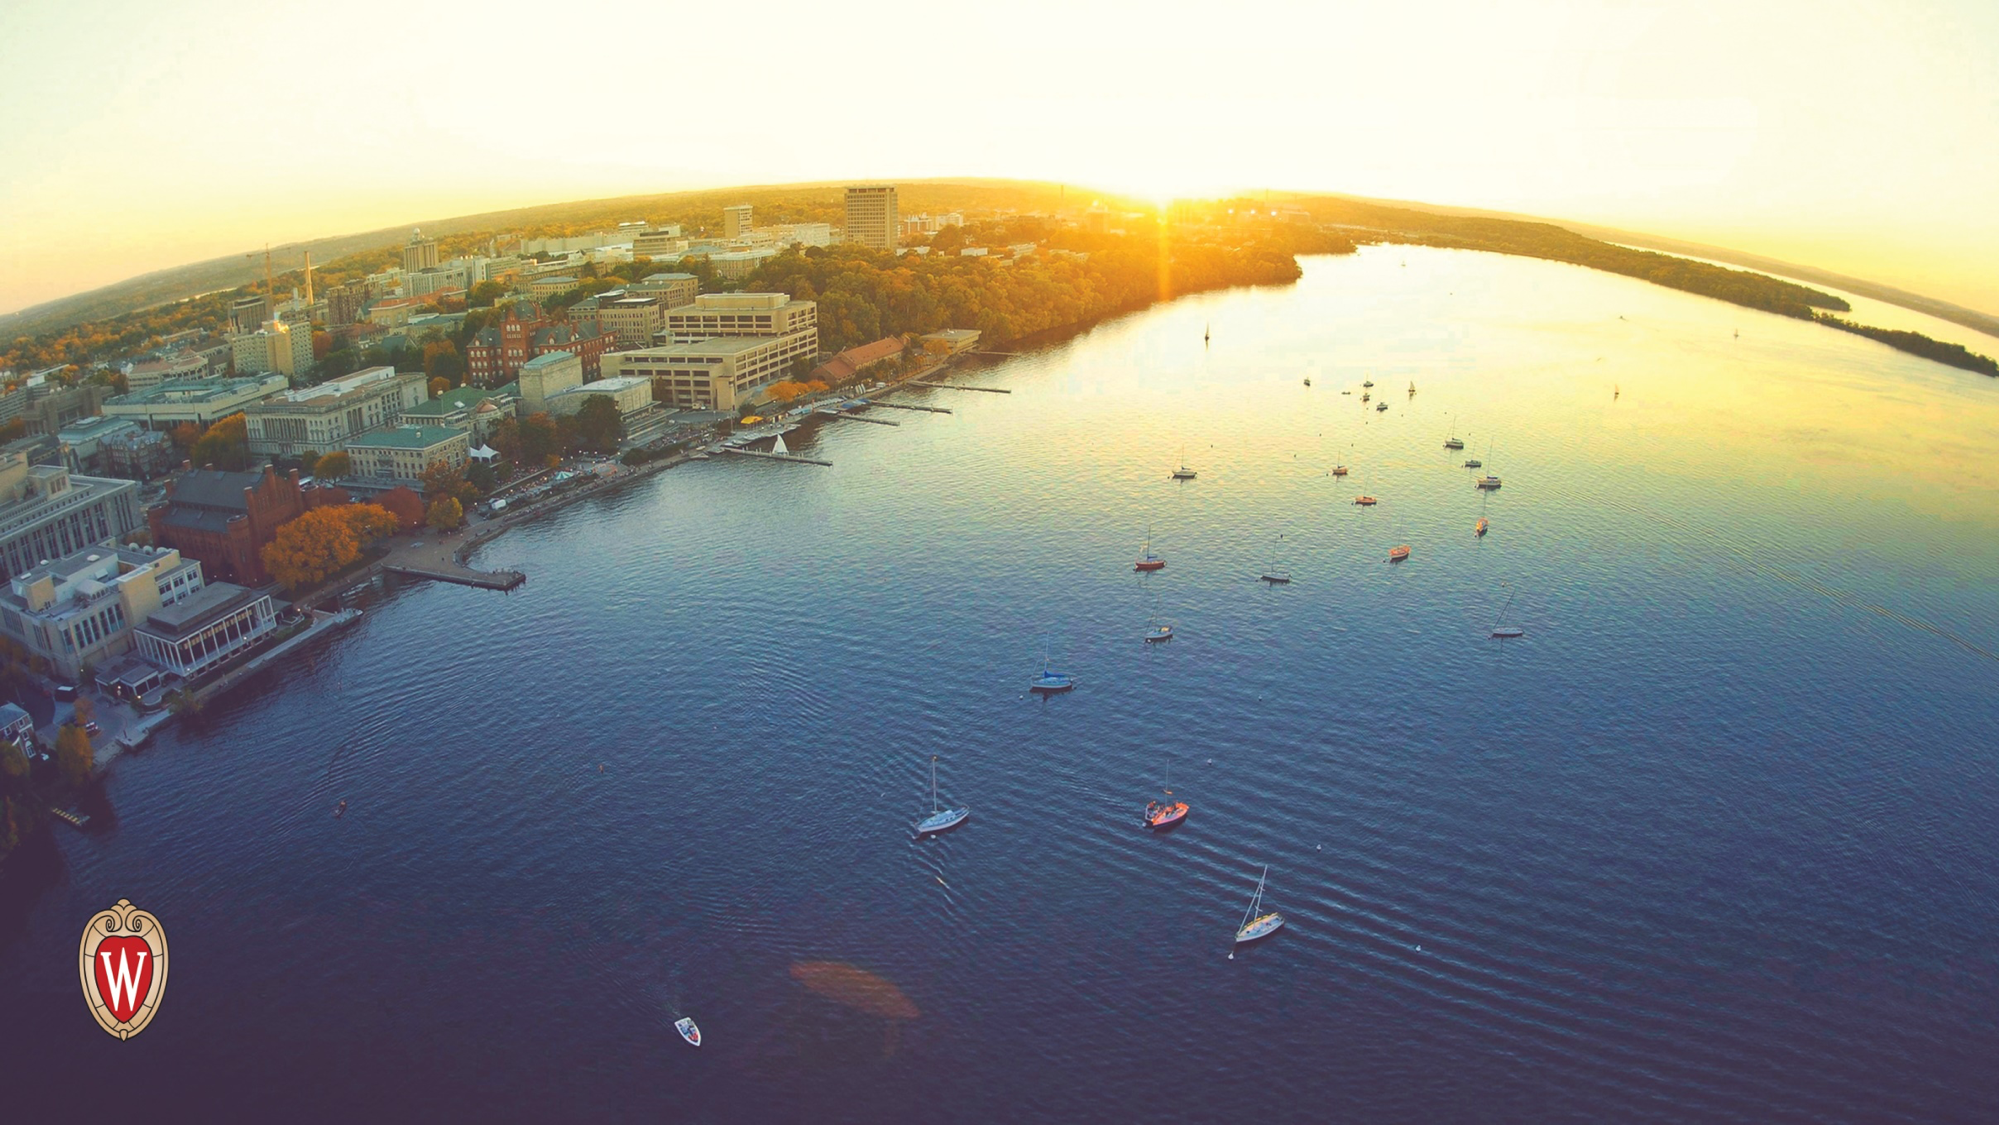
\includegraphics[width=\paperwidth]{UW-lake.png}}
    \begin{frame}[plain]
      \vskip4cm
      \titlepage
    \end{frame}
  }
  
  \section{A section} % This template doesn't do anything for sections

  \begin{frame}{Sample slide}
      \begin{block}{A block}
        Text, \alert{alert text}, etc.
      \end{block}
      \begin{itemize}
        \item Bullet
        \item Points
      \end{itemize}
  \end{frame}

\end{document}